\documentclass{tufte-handout}
\usepackage{graphicx}
\graphicspath{ {./images/} }

\title{Clustering}
\author{Andr\'es Ponce}

\begin{document}
\maketitle

%modify this plz :'(
\begin{abstract}
	Here we study \textit{clusters} of data and how we can use them
	to our advantage.
\end{abstract}

\section{Supervised vs. Unsupervised Learning}
	\subsection{Supervised Learning}
		Using supervised learning, we always have access to the actual 
		answer which we use to compare. For example, we would have an 
		input vector $\mathbf{x}$ and a target vector $\mathbf{t}$,
		then we can see how far off a potential guess is from the actual
		answer. We can see how accurate a model is in predicting the values
		of a function or how accurately a model classifies data. The important
		thing is that we also have a target vector.

		The goal of supervised learning is to learn a \textbf{mapping} between
		the input vector and the target vector (or as close to target vector as 
		possible.)
		
	\subsection{Unsupervised Learning}
		For unsupervised learning, we only have access to $\mathbf{x}$, the 
		input data vector. 
		The goal of unsupervised learning is to then find a \textbf{relation} or
		otherwise hidden structure in the data. Some common use cases for
		unspupervised learning include: clustering, dim. reduction, density estimation,
		data generation, etc...

\section{Unsupervised Learning applications}
	\subsection{Clustering}
		\begin{marginfigure}
			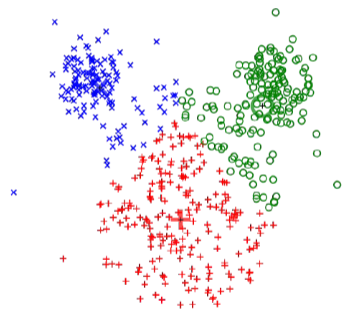
\includegraphics[scale=0.4]{kmeans.png}
			\caption{We split the data set into $k$ clusters. 
				Data points in each cluster	are more similar to each other than to points in other clusters.
			}			
		\end{marginfigure}

		\textbf{Goal}: given a data set, separate the data into \textbf{clusters}, or regions 
		where many data points gather. 
		The points in these areas are more similar to themselves than they are to members
		of other clusters.

	\subsection{Dimensionality Reduction}
		Similar to the second homework assignment, we take a data set with $k$ dimensions of data and try 
		to project it onto a lower data space. 
		This reduces the complexity of solving problems on this data.

	\subsection{Density Estimation}
		Given a set of data points, try to find a probability density function.

	\subsection{Data reconstruction}
		Build models that can efficiently \textbf{encode} and \textbf{decode} the data once its sent.
		The encoder decreases the dimensionality of the data, whereas the decoder will increase the 
		dimensionality to reconstruct the original data.

	\subsection{Data generation}
		Here we can generate new images from a high dimensional distribution.
		\footnote{Is this how the NVIDIA program generated new faces?}

\section{Clustering}
	As mentioned, these types of problems ask us to find related groups of data points in $D$ dimensional
	data.
	We introduce the dimensional vectors $\mu_{k}$ for each of the $k$ clusters.
	These vectors are directed at the center of the data points in the cluster.
	The objective is to find the configuration such that the sum of squares distance between each data point
	and its vector is at a minimum.
	We also have an indicator variables $r_{nk}\in \{0,1\}$ if $\mathbf{x_{n}}$ is assigned to the $k$-th cluster.
	
	For clustering, the objective function is called a \textbf{distortion measure}, and is represented by 
	\footnote{ This equation basically sums the squared distance between a data point if it is assigned to 
		cluster $k$ and all the dimensional vectors. I guess we try to find the configuration such that this 
		is minimized?
	}
	\[ J = \sum_{n=1}^{N}\sum_{k=1}^{K}r_{nk}\|\mathbf{x_{n}} - \mu_{k}\|^{2}\]

	The main steps in the k-clustering algorithm can be summarized as follows:
	\begin{enumerate}
		\item Choose some initial values for clusters $\mu_{k}$
		\item Keep the clusters $\{\mu_{k}\}_{k=1}^{k}$ fixed and try to minimize $J$ w.r.t. assignment
				$\{\mu_{k}\}_{k=1}^{K}$
		\item Keep assignment $\{\mu_{k}\}_{k=1,n=1}^{K,N}$ fixed and minimize $J$ w.r.t. clusters 
				$\{\mu_{k}\}$
		\item Repeat steps 2 and 3 until convergence.
	\end{enumerate}

	This algorithm is really more reflective of a broader type of algorithms: \textbf{Expectation-Maximization}
		algorithms.
	These algorithms consists of two steps:
	We then continuously keep modifying our prediction for $\mu_{k}$ for each k, either by using the entire
		set of points for a cluster or only a subset. 
	Similar to what we did in homework 1, we can adjust the new dimensional vector with the formula:
	\[u_{k}^{new} = u_{k}^{old} + \eta_{n}(x_{n} - \mu_{k}^{old})\]

	\subsection{$k$-medoids clustering}
	This clustering method is the same as the regular $k$-means except that:
	\begin{enumerate}
			\item The objective function is now 
					\[\overline{J} = \sum_{n=1}^{N}\sum_{k=1}^{K}r_{nk}V(x_{n}, \mu_{k})\]
					This new objective function allows us to generalize so we are not required to use 
					Euclidean distance as a measure of dissimlarity. 
					Using a straightforward Euclidean distance could make our estimates susceptible to outliers.

			\item Now in the  M-step, $\mu_{k}$ has to be a data point. We set $\mu_{k}$ eqaul to the data point
					with the shortest average distance to all other points.
	\end{enumerate}
	Notice that $k$-medoids could be quite expensive to run, since we have to evaluate $V$ every iteration for
	every data point.

	\subsection{Image segmentation using k-means clustering}

	The objective of $k$-means clustering on images is to separate them into regions whose pixels have similar
		appearance.
	One big use case for image segmentation would be compression.
	However, there are some diffrences from what we have mentioned: since we are working with images, our 
		input vector $\mathbf{x_{n}}$ is comprised of values $\in\{0,1\}$, so we are not finding the Euclidean
		distance necessarily.
	We could apply this to do \textbf{lossless} compression or \textbf{lossy} compression, where we do not
		allow any missing informationn for the original image values and where we allow an acceptable amount,
		respectively. 
	With lossy compression, we could set each individual image value to the value of its nearest $\mu_{k}$.

	\subsection{Gaussian Distribution}
	To remind, a probability distribution is \textbf{Gaussian} if values vollow the formula
	\footnote{Here $\mu$ is the mean vector and $\Sigma$ is the covariance matrix}
	\[ 
		\mathcal{N}(x|\mu, \Sigma) = \frac{1}{(2\pi)^{D/2}}\frac{1}
		{|\Sigma|^{1/2}}\textrm{exp}\{-\frac{1}{2}(x - \mu)^{T}\Sigma^{-1}(x - \mu)\}
	\]
	Although Gaussian distributions appear quite frequently in nature (e.g. heights and weights of populations)
		or in more human situations (e.g. testing scores), some patterns of data are not fit to be described
		by a Gaussian distribution.

	%% Unfit Gaussian image
	\begin{marginfigure}
			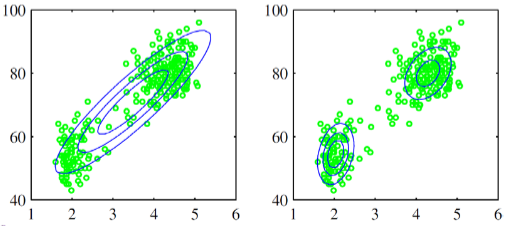
\includegraphics[scale=0.3]{gaussian}
			\caption{These distributions do not reflect the standard ``bell curve" normally associated with 
				Gaussian distributions.}
	\end{marginfigure}

	\subsection{Gaussian Mixture Model}
	In the context of clustering, for $k$ clusters we could have up to $k$ different Gaussian distributions 
		controlling the data points that belong to that cluster.

	We introduce a variable $z$ such that for each data point $\mathbf{x}_{n}$, there is also a $z_{n}$. 
	Also $z\in\{0,1\}$ and $\sum_{k}^{} z_{k}= 1$. 
	\footnote{This means that for every $x_{n}$, it will have a value such that z indicates which group it
		belongs to. From the classification section, this is a \textbf{1-of-k} representation.}

	Thus to calculate the probability $\mathbf{x}$ belongs to a certain cluster, we have to calculate the 
	joint and marginal probability of x and z. 

	The probability $\mathbf{z}$ is equal to 1 depends on the \textbf{mixing coefficient} of the distributions,
	or how separated they are. 
	The marginal probability of $\mathbf{z}$ is expressed by
	\[ p(\mathbf{z}) = \prod_{k=1}^{K}\pi^{z_{k}}_{k}\]
	
	The conditional probability $p(x|\mathbf{z})$ would then be the product of 
		$\mathcal{N}(x|\mu_{k},\Sigma_{k})$.

	We have already modeled the conditional probability that $mathbf{z} = 1$ given $\mathbf{x}$, and now
		we model the other conditional probability: $p(\mathbf{z}|x)$.
	This term $\gamma$ we call the \textbf{responsibility} that $k$ takes for explaining x. 
	Although the formula is complicated, it is not hard:
	\footnote{What this formula essentially says is that the probability that $z$ is correct given $x$
		is equal to the probability $x$ belongs to cluster $k$ over the probability that it belongs
		to any other cluster.
	}
	\[ \gamma(z_{k}) = \frac{p(z_{k = 1})p(x|z_{k} = 1)}
		{\sum_{j = 1}^{K}\pi_{j}\mathcal{N}(x|\mu_{j},\Sigma_{j})}
	\]


\end{document}
